\section{Development model}
The workflow for the development is show in figure
\ref{fig:gajski-kuhn-ychart}. In the Gajski-Kuhn Y-model has 3 axis for the
perspectives of the product. It is typical to start from the behavioral axis,
by treating the systems as a black-box, and then to jump back and forth between
the other axis while gravitating towards the origin (project goal).
\begin{figure}[h]
  \centering
  \resizebox{\linewidth}{!}{
    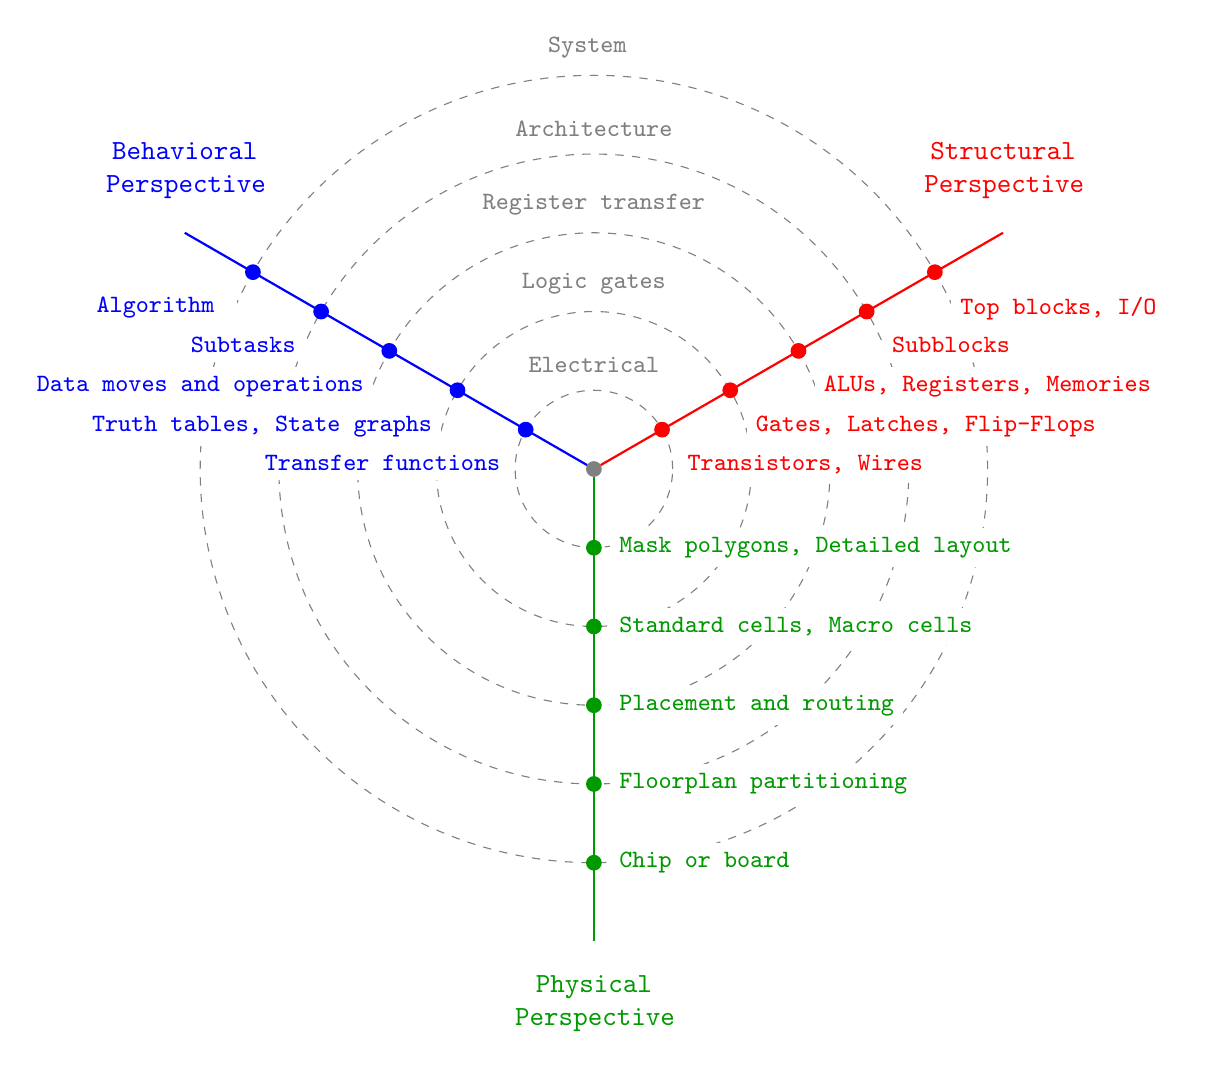
\begin{tikzpicture}[
        font=\ttfamily,
      ]
      \draw[gray] node[
        circle,
        fill = gray,
        minimum size = 2mm,
        outer sep = 0,
        inner sep = 0,
      ] (O) at (0,0) {};

      \foreach \r/\desc in {
        1/{Electrical},
        2/{Logic gates},
        3/{Register transfer},
        4/{Architecture},
        5/{System}
      }{
        \draw[gray, dashed] (O) circle (\r);
        \draw[gray] (90:\r)
          node[
            above = 1mm,
            align = center,
            font = \small\ttfamily,
            fill = white,
          ] {\desc};
      }

      \draw[red, thick] (O) to ++(30:6)
        node[
          above = 3mm,
          align = center,
          text width = 2cm
        ] {\textbf{Structural Perspective}};
      \foreach \r/\desc in {
        1/{Transistors, Wires},
        2/{Gates, Latches, Flip-Flops},
        3/{ALUs, Registers, Memories},
        4/{Subblocks},
        5/{Top blocks, I/O}
      } {
        \draw[red] (30:\r)
          node[
            circle, minimum size = 2mm,
            fill = red,
            outer sep = 0,
            inner sep = 0
          ] {}
          node[
            below right = 2mm,
            align = left,
            font = \small\ttfamily,
            fill = white,
          ] {\desc};
      }

      \draw[blue, thick] (O) to ++(150:6)
        node[
          above = 3mm,
          align = center,
          text width = 2cm
        ] {\textbf{Behavioral Perspective}};
      \foreach \r/\desc in {
        1/{Transfer functions},
        2/{Truth tables, State graphs},
        3/{Data moves and operations},
        4/{Subtasks},
        5/{Algorithm}
      } {
        \draw[blue] (150:\r)
          node[
            circle, minimum size = 2mm,
            fill = blue,
            outer sep = 0,
            inner sep = 0
          ] {}
          node[
            below left = 2mm,
            align = right,
            font = \small\ttfamily,
            fill = white,
          ] {\desc};
      }

      \draw[green!60!black, thick] (O) to ++(270:6)
        node[
          below = 3mm,
          align = center,
          text width = 2cm
        ] {\textbf{Physical Perspective}};
      \foreach \r/\desc in {
        1/{Mask polygons, Detailed layout},
        2/{Standard cells, Macro cells},
        3/{Placement and routing},
        4/{Floorplan partitioning},
        5/{Chip or board}
      } {
        \draw[green!60!black] (270:\r)
          node[
            circle, minimum size = 2mm,
            fill = green!60!black,
            outer sep = 0,
            inner sep = 0
          ] {}
          node[
            right = 2mm,
            align = left,
            font = \small\ttfamily,
            fill = white,
          ] {\desc};
      }

    \end{tikzpicture}
  }
  \caption{
    Gajski-Kuhn Y-chart.
    \label{fig:gajski-kuhn-ychart}
  }
\end{figure}

%% TODO: finish picture
\iffalse
Figure \ref{fig:asic-design-flow} shows a typical flow diagram of how an ASIC device
is designed.
\begin{figure}[h]
  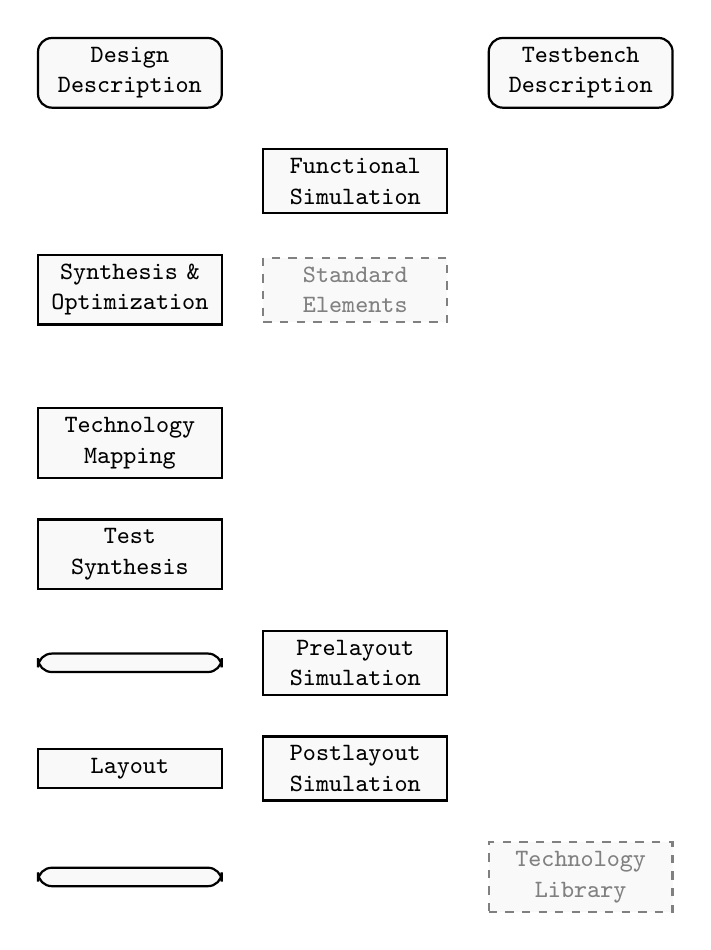
\begin{tikzpicture}[
      scale = .7,
      font = \small\ttfamily,
      bubble/.style = {
        rectangle,
        draw = black, thick,
        fill = lightgray!10,
        align = center,
        text width = 2.1cm,
        rounded corners = 5pt,
      },
      box/.style = {
        rectangle,
        draw = black, thick,
        fill = lightgray!10,
        align = center,
        text width = 2.1cm,
      },
      lib/.style = {
        rectangle,
        draw = black, gray, thick, dashed,
        fill = lightgray!10,
        align = center,
        text width = 2.1cm,
      },
      ghost/.style = {
        outer sep = 0,
        inner sep = 0,
      }
    ]
    \matrix[row sep = 5mm, column sep = 5mm]{
      \node[bubble] (dd) {Design Description}; & & \node[bubble] (tbd) {Testbench Description}; \\
      \node[ghost] (A) {}; & \node[box] (fs) {Functional Simulation}; \\
      \node[box] (so) {Synthesis \& Optimization}; & \node[lib] (se) {Standard Elements}; \\
      \node[ghost] (lineA) {}; & & \node[ghost] (lineB) {}; \\
      \node[box] (tm) {Technology Mapping}; \\
      \node[box] (ts) {Test Synthesis}; \\
      \node[bubble] (gates) {}; & \node[box] (pres) {Prelayout Simulation}; \\
      \node[box] (l) {Layout}; & \node[box] (posts) {Postlayout Simulation}; \\
      \node[bubble] (design) {}; & & \node[lib] {Technology Library}; \\
    };
  \end{tikzpicture}
  \caption{
    Design flow for an ASIC device.
    \label{fig:asic-design-flow}
  }
\end{figure}
\fi

% \section{Hardware}
